\documentclass{article}
\usepackage{amsmath,amssymb}
\usepackage{xcolor}
\usepackage{graphicx}        
\graphicspath{{./}{images/}} 
\usepackage{geometry}
\geometry{a4paper, margin=1in}

\title{Modified Euler–Bernoulli Beam Theory with Axial Displacement:\\Linear axial interpolation}

\begin{document}
	\maketitle
	
	\section{Introduction}
	The classical Euler–Bernoulli beam theory models only transverse displacement \(w(x,t)\) and rotation
	\[
	\theta(x,t) \;=\; \frac{\partial w}{\partial x}.
	\]
	To extend this model, we add an axial displacement \(u(x,t)\) as an additional degree of freedom.  This allows the beam to deform both in bending and in axial stretch simultaneously.
	
	\section{Degrees of freedom and physical meaning}
	Each node in the extended model carries three DOFs:
	\[
	u\quad(\text{axial}),\quad
	w\quad(\text{transverse}),\quad
	\theta\quad(\text{rotation}).
	\]
	A two-node element therefore has the local vector
	\(\{u_1,\,w_1,\,\theta_1,\,u_2,\,w_2,\,\theta_2\}^T\).
	
	\section{Shape functions}
	\subsection{Axial displacement \(u(x)\)}
	We use linear interpolation over an element of length \(L_e\):
	\[
	u(x) \;=\; N^{(u)}_1(x)\,u_1 \;+\; N^{(u)}_2(x)\,u_2,
	\quad
	N^{(u)}_1=1-\frac{x}{L_e},\quad
	N^{(u)}_2=\frac{x}{L_e}.
	\]
	
	\subsection{Transverse displacement \(w(x)\)}
	We use Hermite cubic polynomials:
	\[
	w(x)
	= N^{(w)}_1(x)\,w_1
	+ N^{(w)}_2(x)\,\theta_1
	+ N^{(w)}_3(x)\,w_2
	+ N^{(w)}_4(x)\,\theta_2,
	\]
	where
	\begin{align*}
		N^{(w)}_1(x) &= 1-3\Bigl(\tfrac{x}{L_e}\Bigr)^2 + 2\Bigl(\tfrac{x}{L_e}\Bigr)^3,\\
		N^{(w)}_2(x) &= x\Bigl(1-2\tfrac{x}{L_e} + \bigl(\tfrac{x}{L_e}\bigr)^2\Bigr),\\
		N^{(w)}_3(x) &= 3\Bigl(\tfrac{x}{L_e}\Bigr)^2 - 2\Bigl(\tfrac{x}{L_e}\Bigr)^3,\\
		N^{(w)}_4(x) &= x\Bigl(-\tfrac{x}{L_e} + \bigl(\tfrac{x}{L_e}\bigr)^2\Bigr).
	\end{align*}
	
	\section{Strain energy of the element}
	The total strain energy is the sum of an axial part and a bending part:
	\[
	U = \frac12 \int_{0}^{L_e} EA\Bigl(\tfrac{du}{dx}\Bigr)^2\,dx
	+ \frac12 \int_{0}^{L_e} EI\Bigl(\tfrac{d^2w}{dx^2}\Bigr)^2\,dx.
	\]
	
	\section{Derivation of element stiffness matrix}
	\subsection{Axial Part}
	Because \(du/dx\) is constant,
	\[
	\varepsilon = \frac{du}{dx} = -\frac{u_1}{L_e} + \frac{u_2}{L_e},
	\]
	one obtains
	\[
	U_{\rm axial}
	= \frac{EA}{2L_e}(u_1^2 - 2u_1u_2 + u_2^2),
	\quad\Longrightarrow\quad
	k^{(\rm axial)} = \frac{EA}{L_e}
	\begin{bmatrix}1 & -1\\[4pt] -1 & 1\end{bmatrix}.
	\]
	
	\subsection{Bending part}
	The standard Hermite–Euler–Bernoulli bending stiffness is
	\[
	k^{(\rm bending)}
	= \frac{EI}{L_e^3}
	\begin{bmatrix}
		12      &  6L_e   & -12     &  6L_e\\[4pt]
		6L_e    &  4L_e^2 & -6L_e   &  2L_e^2\\[4pt]
		-12      & -6L_e   &  12     & -6L_e\\[4pt]
		6L_e    &  2L_e^2 & -6L_e   &  4L_e^2
	\end{bmatrix}.
	\]
	
	\section{Full element stiffness matrix}
	Placing the \(2\times2\) axial block in the \(\{u_1,u_2\}\) rows and cols,
	and the \(4\times4\) bending block in the \(\{w_1,\theta_1,w_2,\theta_2\}\) rows and cols,
	gives the full \(6\times6\) matrix
	\[
	k_e =
	\begin{bmatrix}
		\frac{EA}{L_e}           & -\frac{EA}{L_e}          & 0               & 0                          & 0                         & 0           \\[6pt]
		-\frac{EA}{L_e}          &  \frac{EA}{L_e}          & 0               & 0                          & 0                         & 0           \\[6pt]
		0                        &  0                        & \tfrac{12EI}{L_e^3} & \tfrac{6EI}{L_e^2}         & -\tfrac{12EI}{L_e^3}      &  \tfrac{6EI}{L_e^2} \\[6pt]
		0                        &  0                        & \tfrac{6EI}{L_e^2}  & \tfrac{4EI}{L_e}           & -\tfrac{6EI}{L_e^2}       &  \tfrac{2EI}{L_e}   \\[6pt]
		0                        &  0                        & -\tfrac{12EI}{L_e^3} & -\tfrac{6EI}{L_e^2}        &  \tfrac{12EI}{L_e^3}      & -\tfrac{6EI}{L_e^2} \\[6pt]
		0                        &  0                        & \tfrac{6EI}{L_e^2}  & \tfrac{2EI}{L_e}           & -\tfrac{6EI}{L_e^2}       &  \tfrac{4EI}{L_e^3}
	\end{bmatrix}.
	\]
	
	\section{Dimensional analysis and units}
	\begin{itemize}
		\item Entries like \(\tfrac{EA}{L_e}\) carry units N/m.
		\item Mixed terms like \(\tfrac{6EI}{L_e^2}\) carry units N.
		\item Pure rotation–rotation terms like \(\tfrac{4EI}{L_e}\) carry units N·m.
	\end{itemize}
	
	\section{Note about radians}
	In SI, radians are dimensionless.  Thus a term such as
	\((EI/L_e)\,\theta\) has units N·m when \(\theta\) is in radians.
	
	\section*{llustration of the beam element}
	\begin{figure}[ht]
		\centering
		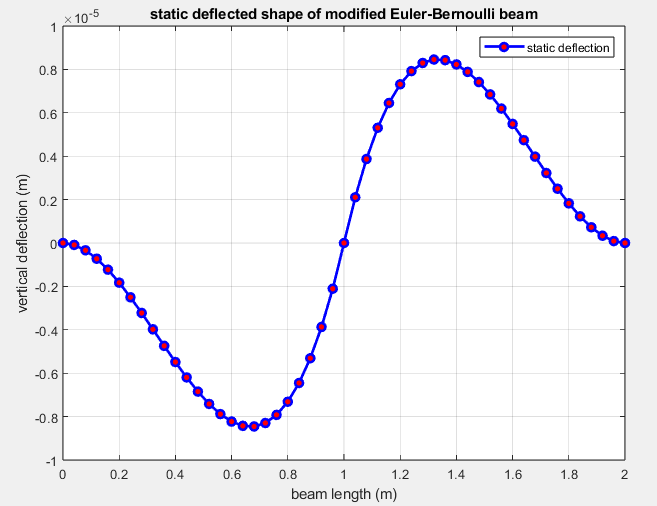
\includegraphics[width=0.8\textwidth]{Linear_Axial.png}
		\caption{Schematic of the deflection extended Euler--Bernoulli beam element by applying moment at the middle of the beam, using linear interpolating function.}
		\label{fig:beam-element}
	\end{figure}
	

\end{document}
